\section{Pengujian Sistem}

Subbab ini menguraikan pengujian aplikasi {data capture} serta pengujian skenario peluncuran model (\textit{model deployment}) melalui simulasi penggunaan aplikasi saat pengguna memasukkan data penyewa ke dalam sistem. Untuk membuktikan kapabilitas model klasifikasi yang telah diintegrasikan, pemaparan pada bagian ini difokuskan pada dua skenario utama, yakni simulasi \textit{input} profil data penyewa normal (aman) dan simulasi \textit{input} data penyewa tidak normal (berpotensi melanggar). Secara keseluruhan, simulasi ini ditampilkan untuk memperlihatkan tahapan pengisian formulir pendataan sewa, eksekusi model terintegrasi, hingga munculnya respons prediksi atau notifikasi dari aplikasi sesaat setelah pengguna menyimpan data.

\newpage
\subsection{Skenario Input Data Penyewa Normal}
Skenario pertama mendemonstrasikan proses pendataan untuk penyewa yang memiliki profil dan pola transaksi wajar. Pada tahap ini, pengguna memasukkan identitas penyewa beserta data pendukung terkait transaksi penyewaan.

\begin{figure}[H]
    \centering
    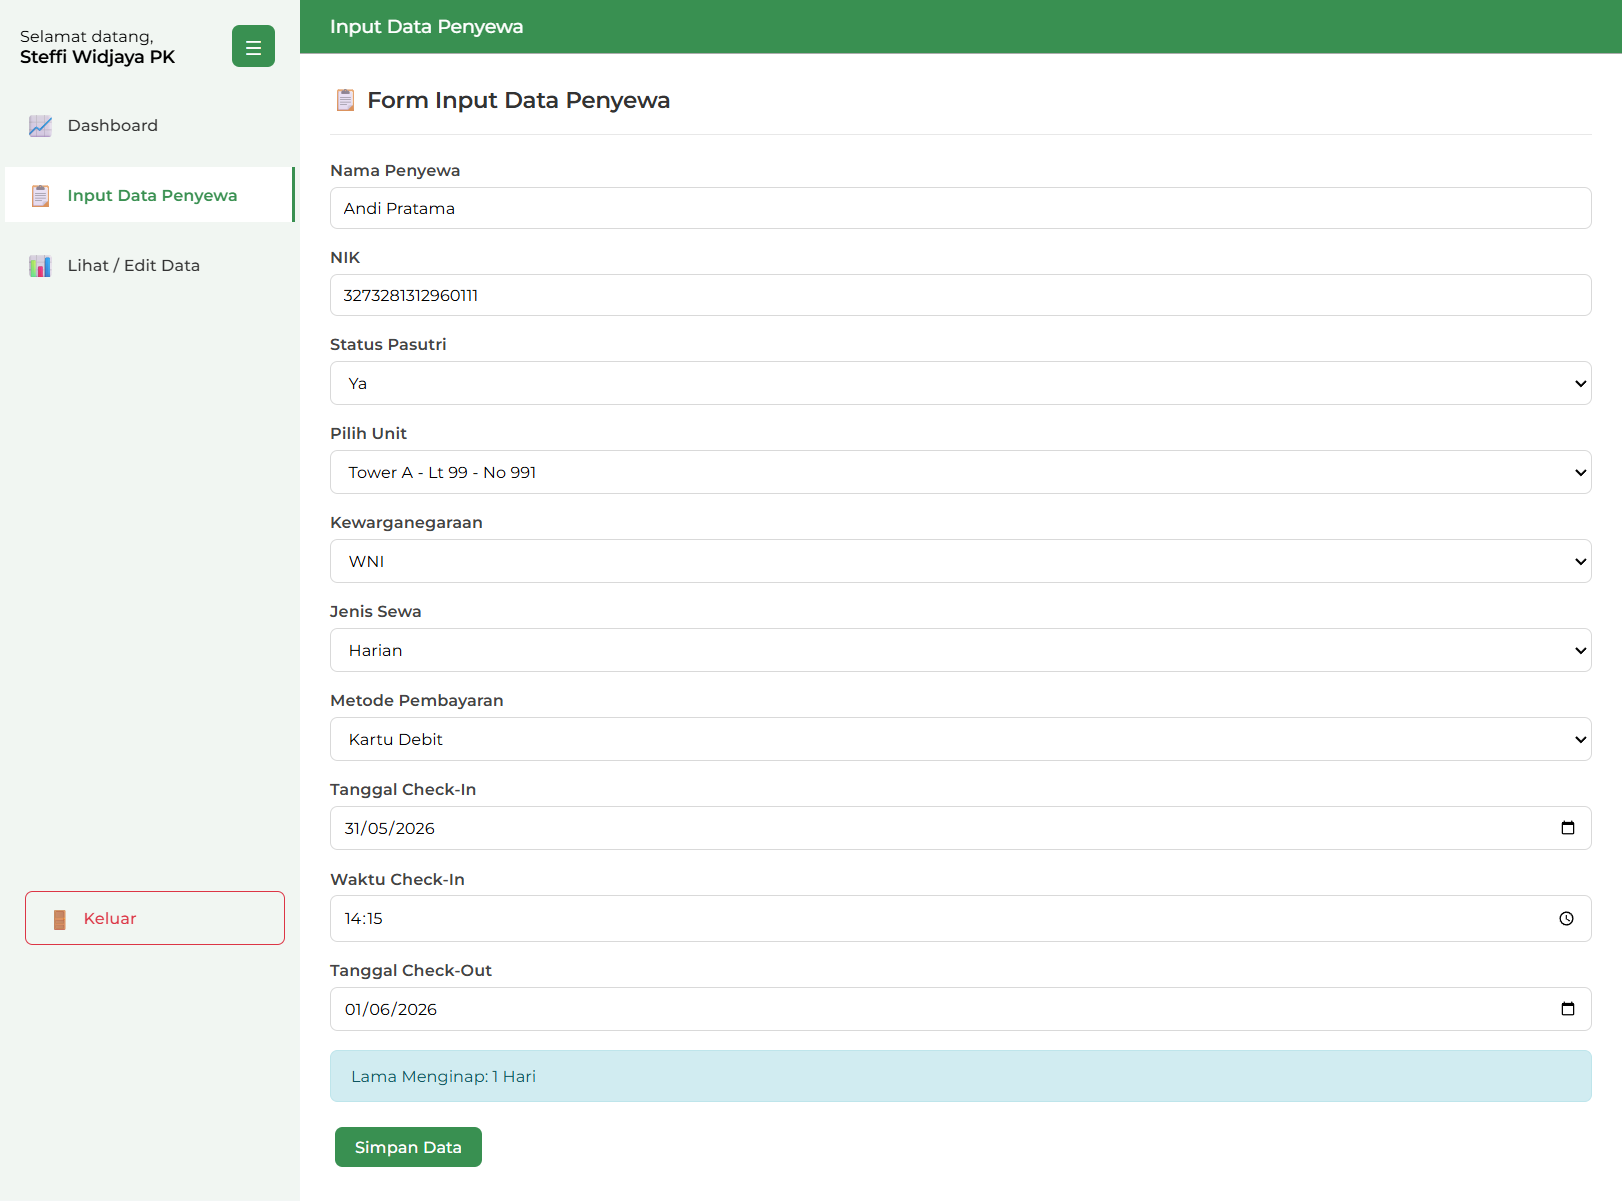
\includegraphics[width=0.7\textwidth]{Gambar/NONmelanggar1a.png} \\
    \vspace{0.2cm}
    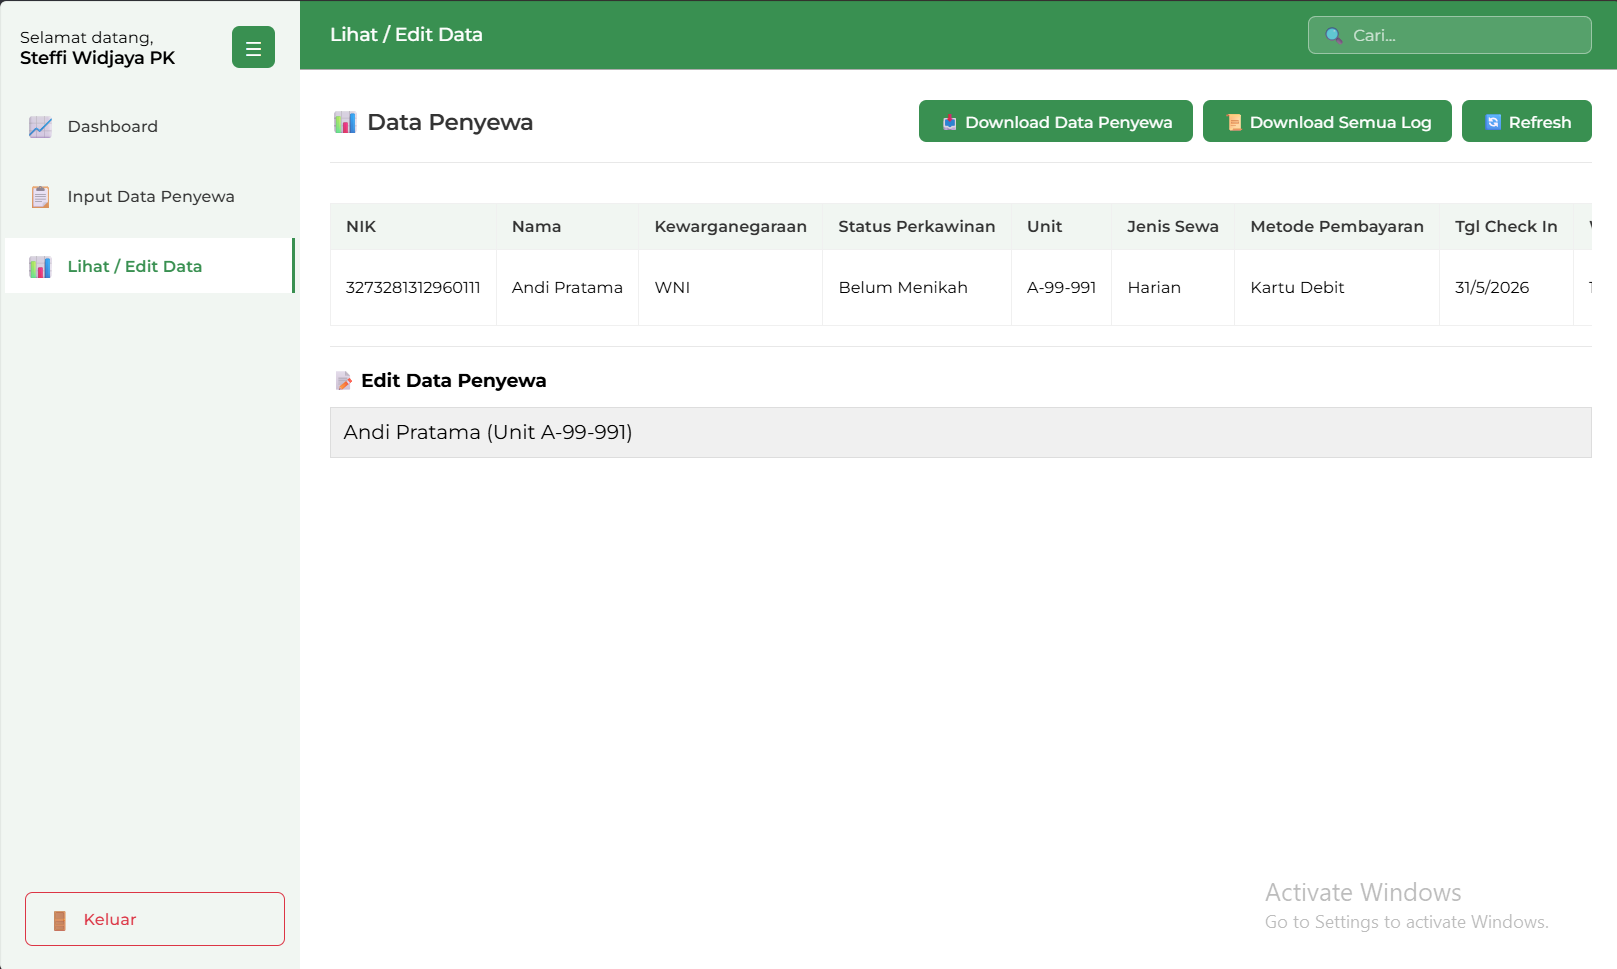
\includegraphics[width=0.7\textwidth]{Gambar/NONmelanggar1b.png}
    \caption{Simulasi Input Data Penyewa Normal (1)}
    \label{fig:sim_input_normal1}
\end{figure}

\begin{figure}[H]
    \centering
    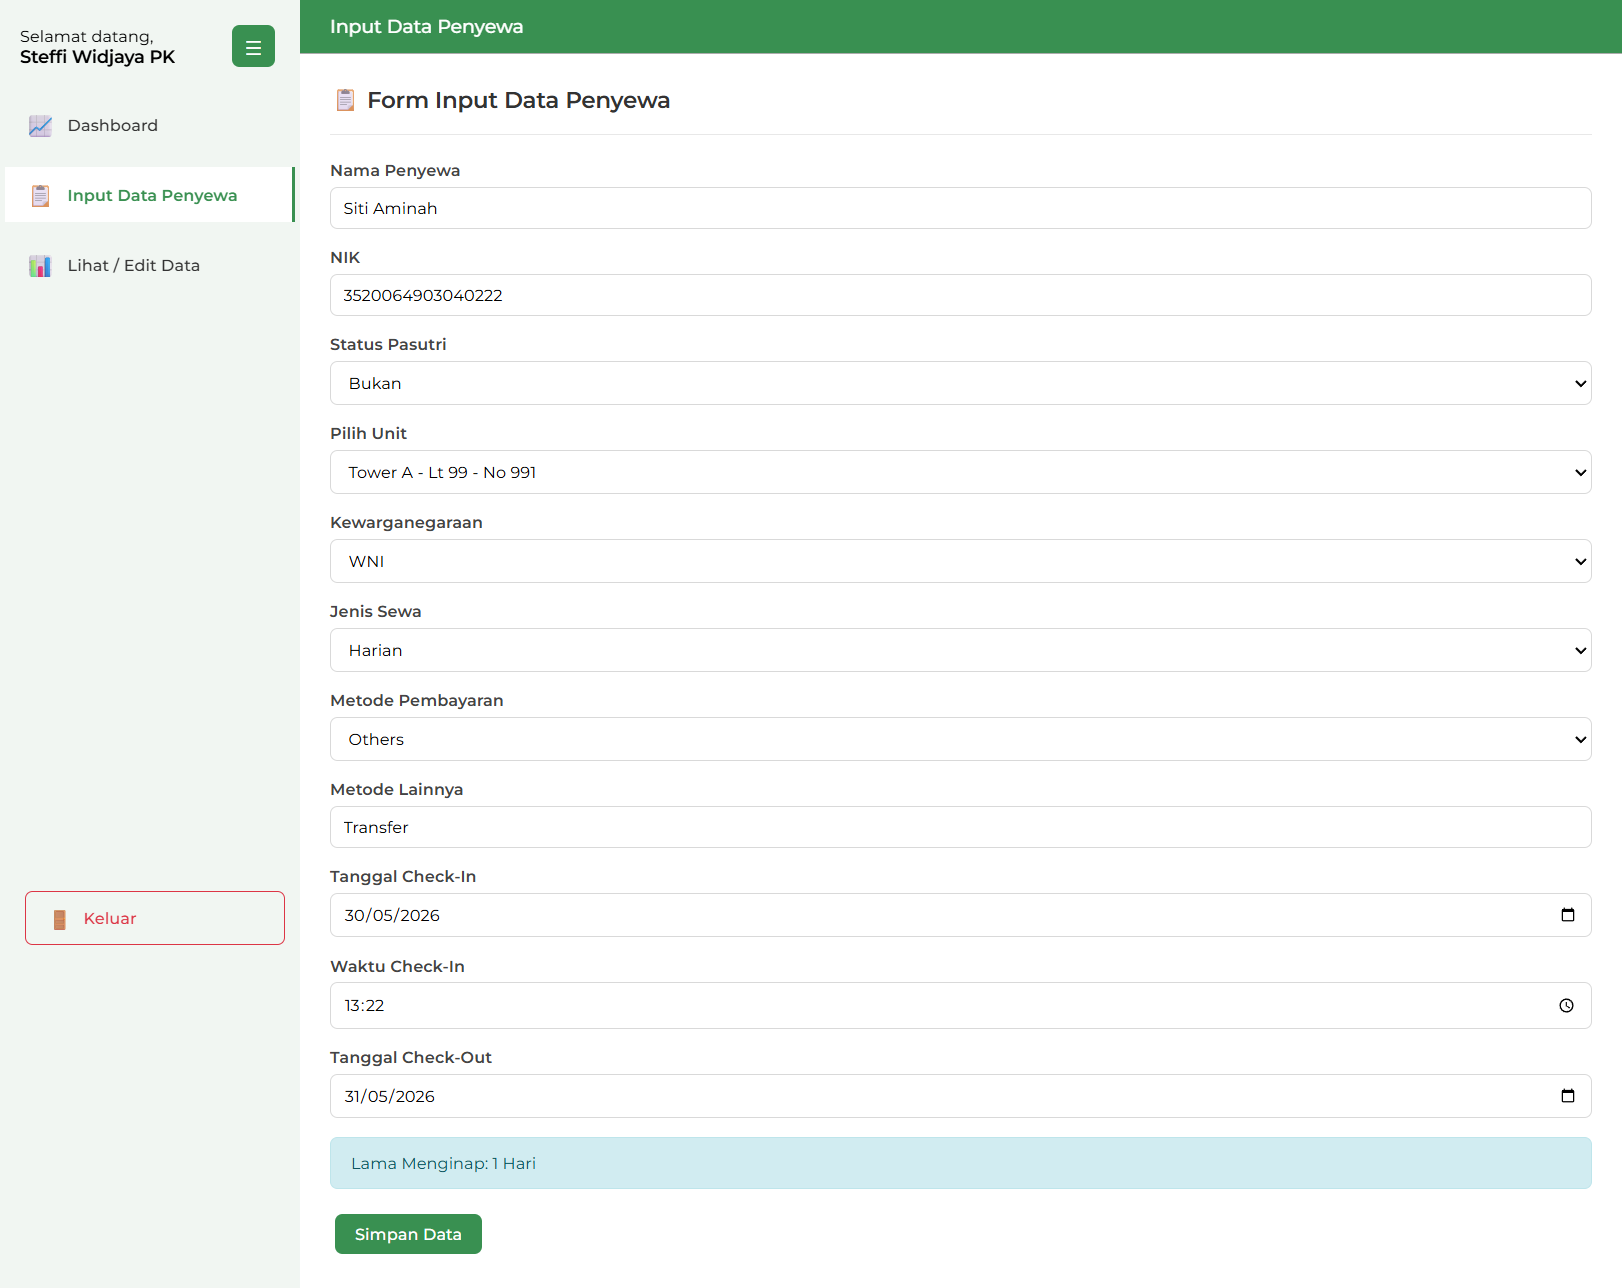
\includegraphics[width=0.7\textwidth]{Gambar/NONmelanggar2a.png} \\
    \vspace{0.2cm}
    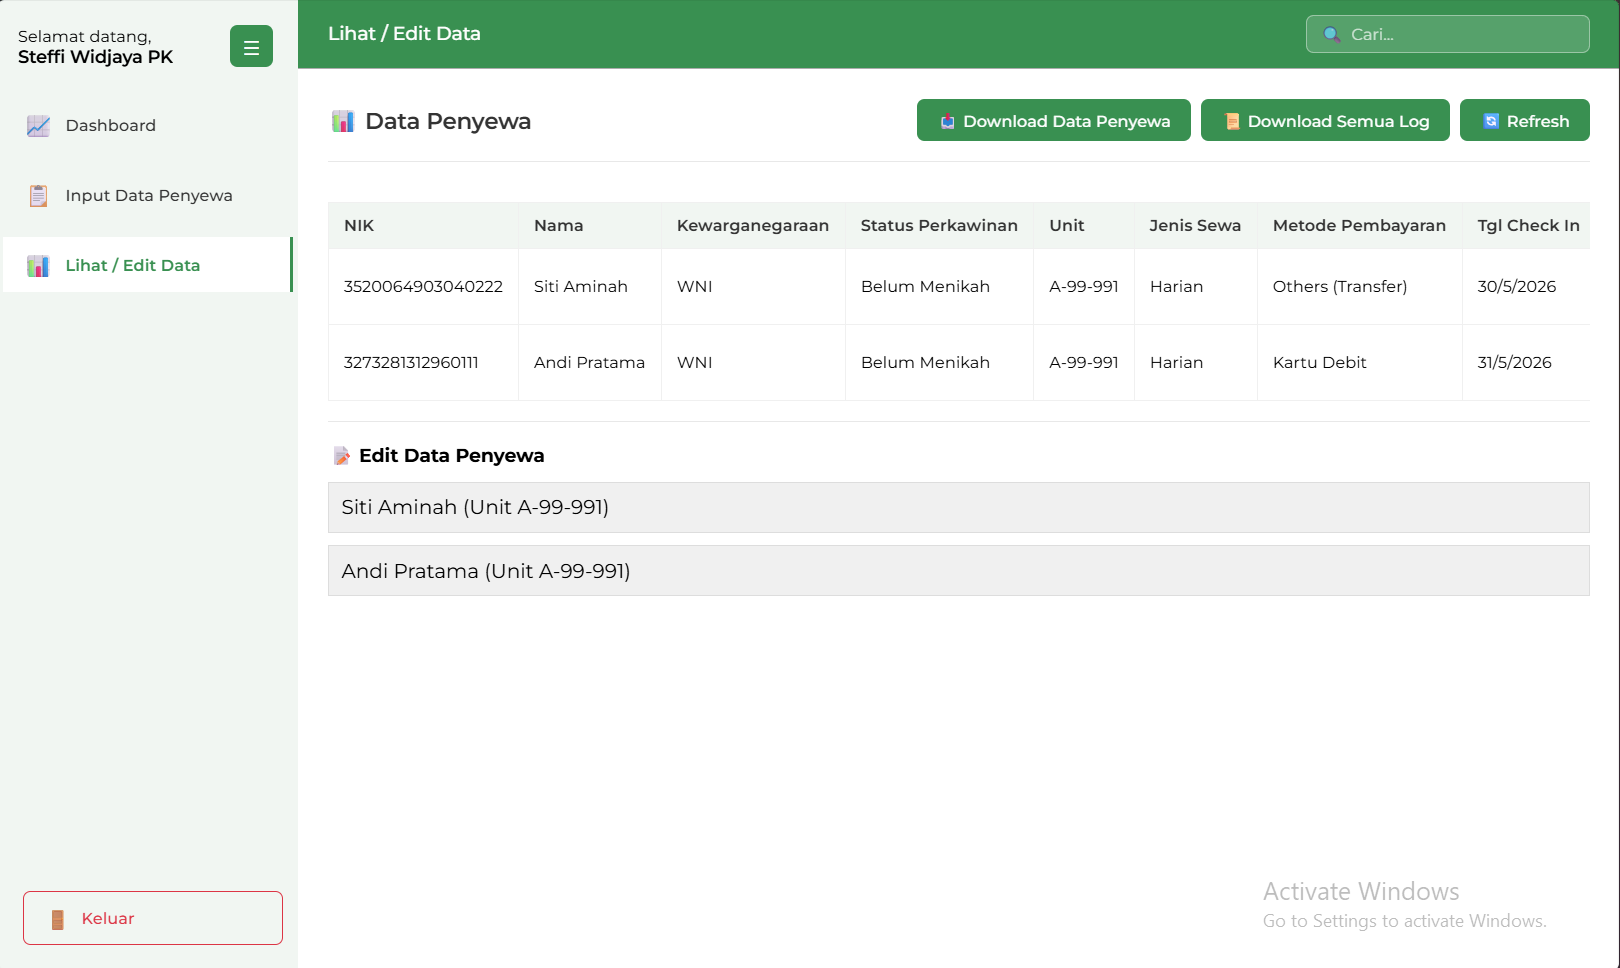
\includegraphics[width=0.7\textwidth]{Gambar/NONmelanggar2b.png}
    \caption{Simulasi Input Data Penyewa Normal (2)}
    \label{fig:sim_input_normal2}
\end{figure}

\begin{figure}[H]
    \centering
    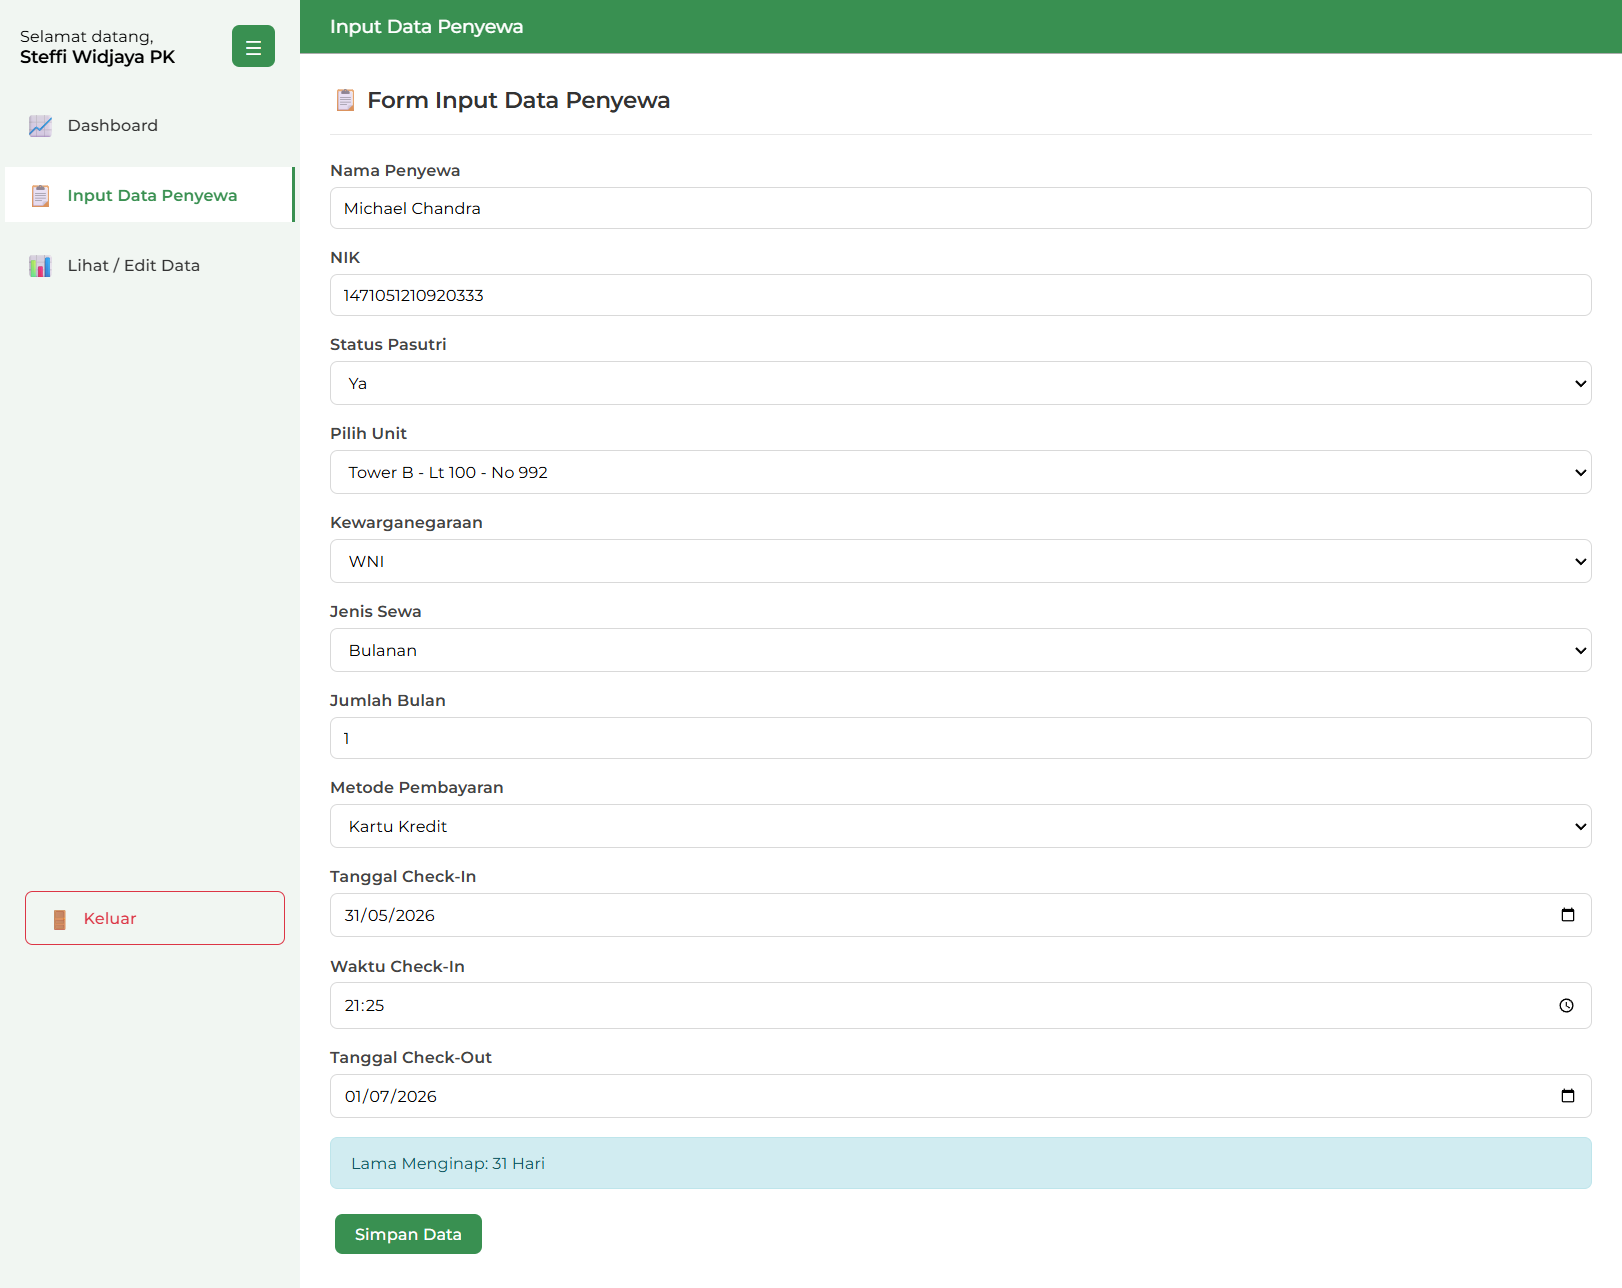
\includegraphics[width=0.7\textwidth]{Gambar/NONmelanggar3a.png} \\
    \vspace{0.2cm}
    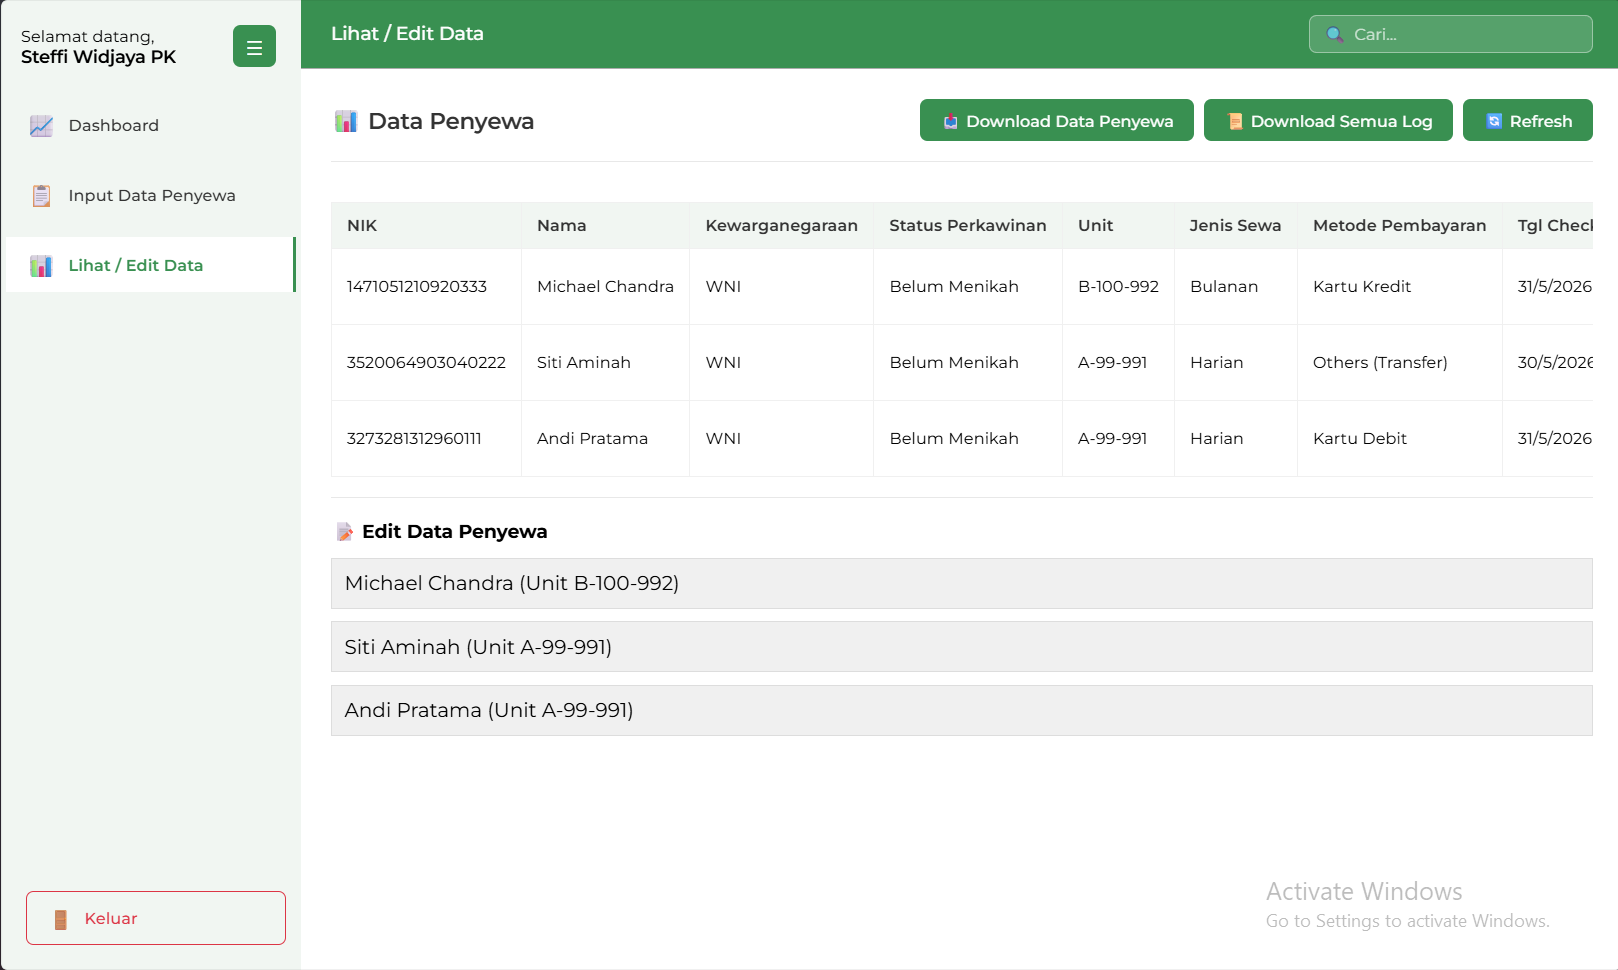
\includegraphics[width=0.7\textwidth]{Gambar/NONmelanggar3b.png}
    \caption{Simulasi Input Data Penyewa Normal (3)}
    \label{fig:sim_input_normal3}
\end{figure}

Gambar~\ref{fig:sim_input_normal1}, \ref{fig:sim_input_normal2}, dan \ref{fig:sim_input_normal3} memperlihatkan pengisian data dengan karakteristik penyewa normal. Parameter yang diinputkan merepresentasikan ciri transaksi yang minim risiko, seperti pemilihan durasi menginap jangka menengah hingga panjang serta kedatangan pada rentang waktu operasional yang wajar. Setelah seluruh kolom formulir dipastikan terisi dengan lengkap, pengguna klik tombol \textit{Simpan Data}. Aplikasi kemudian mengeksekusi data tersebut ke dalam model klasifikasi. Karena profil transaksi yang dikirimkan terindikasi aman (terklasifikasi ke dalam kelas 0), aplikasi memproses dan menyimpan data tersebut langsung ke dalam basis data, tanpa memunculkan notifikasi peringatan apa pun pada layar antarmuka pengguna.

\newpage
\subsection{Skenario Input Data Penyewa Tidak Normal}
Skenario kedua mendemonstrasikan pengisian formulir untuk profil penyewa yang terindikasi memiliki potensi pelanggaran aturan. Sama halnya dengan skenario sebelumnya, pengguna menginputkan informasi identitas dan detail transaksi ke dalam formulir pendataan.

\begin{figure}[H]
    \centering
    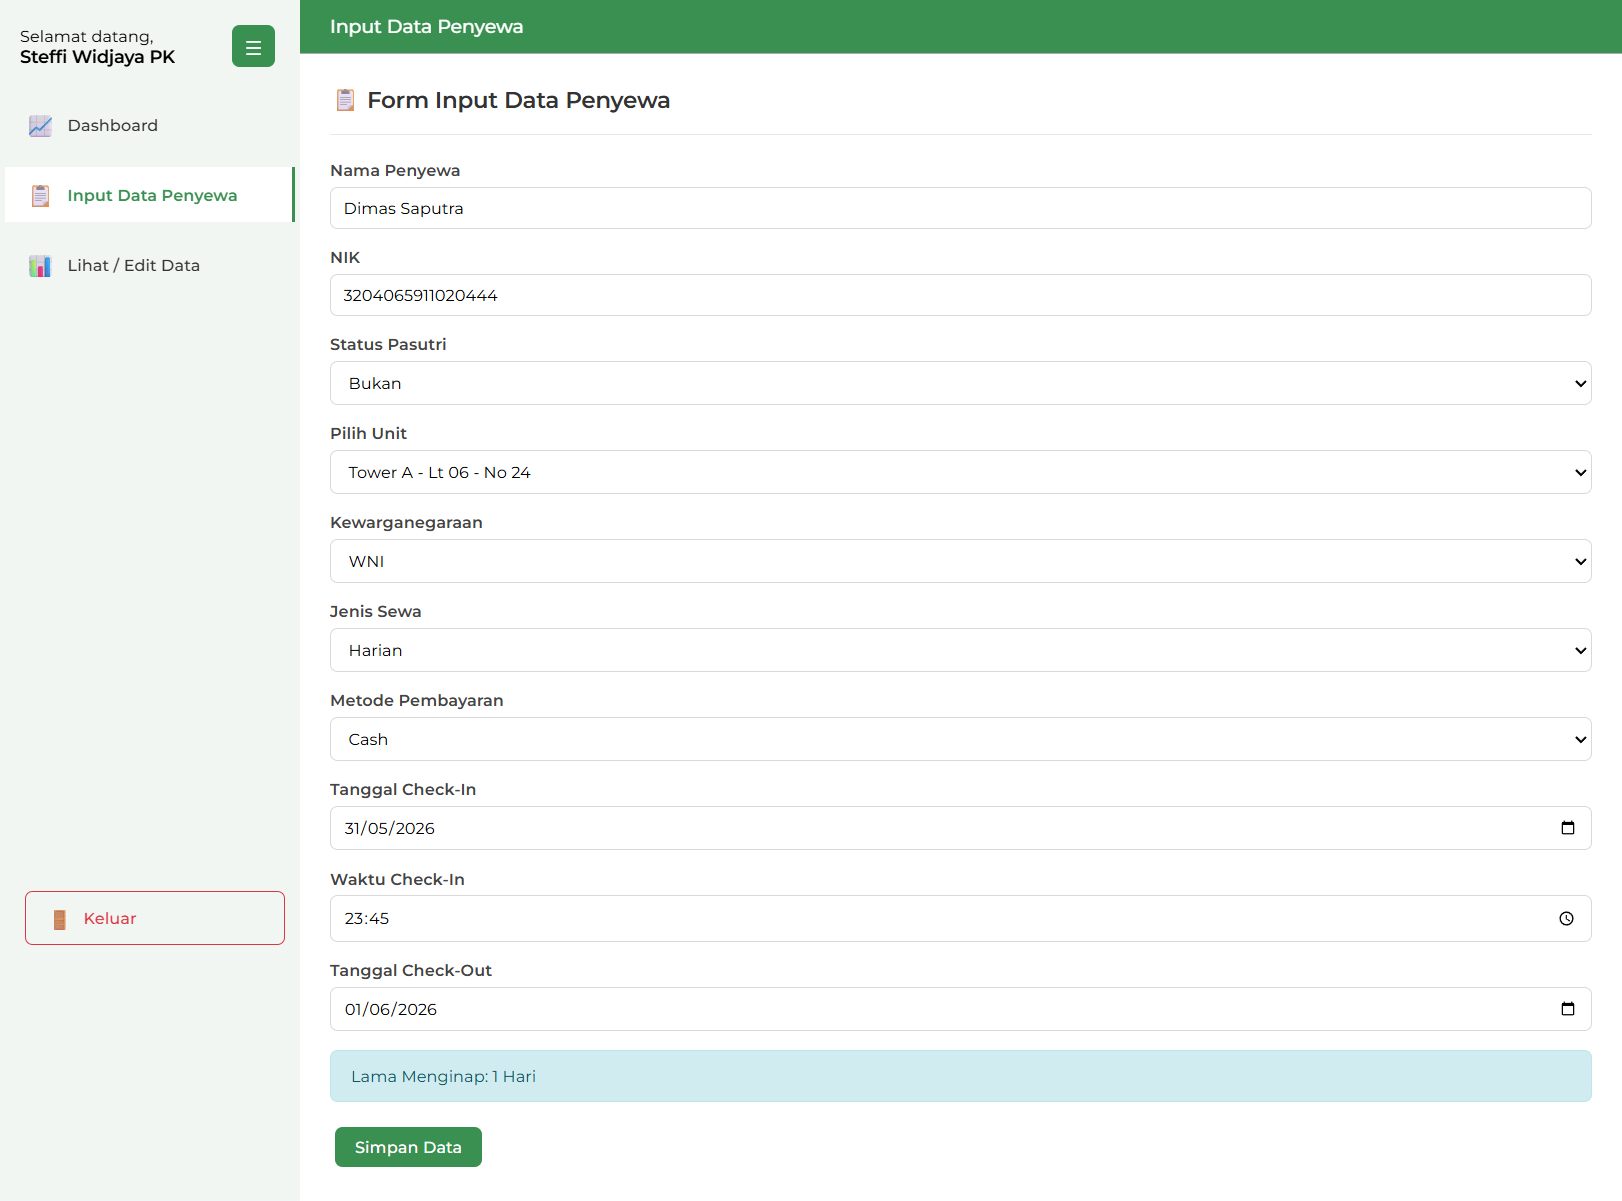
\includegraphics[width=0.7\textwidth]{Gambar/melanggar1a.png} \\
    \vspace{0.2cm}
    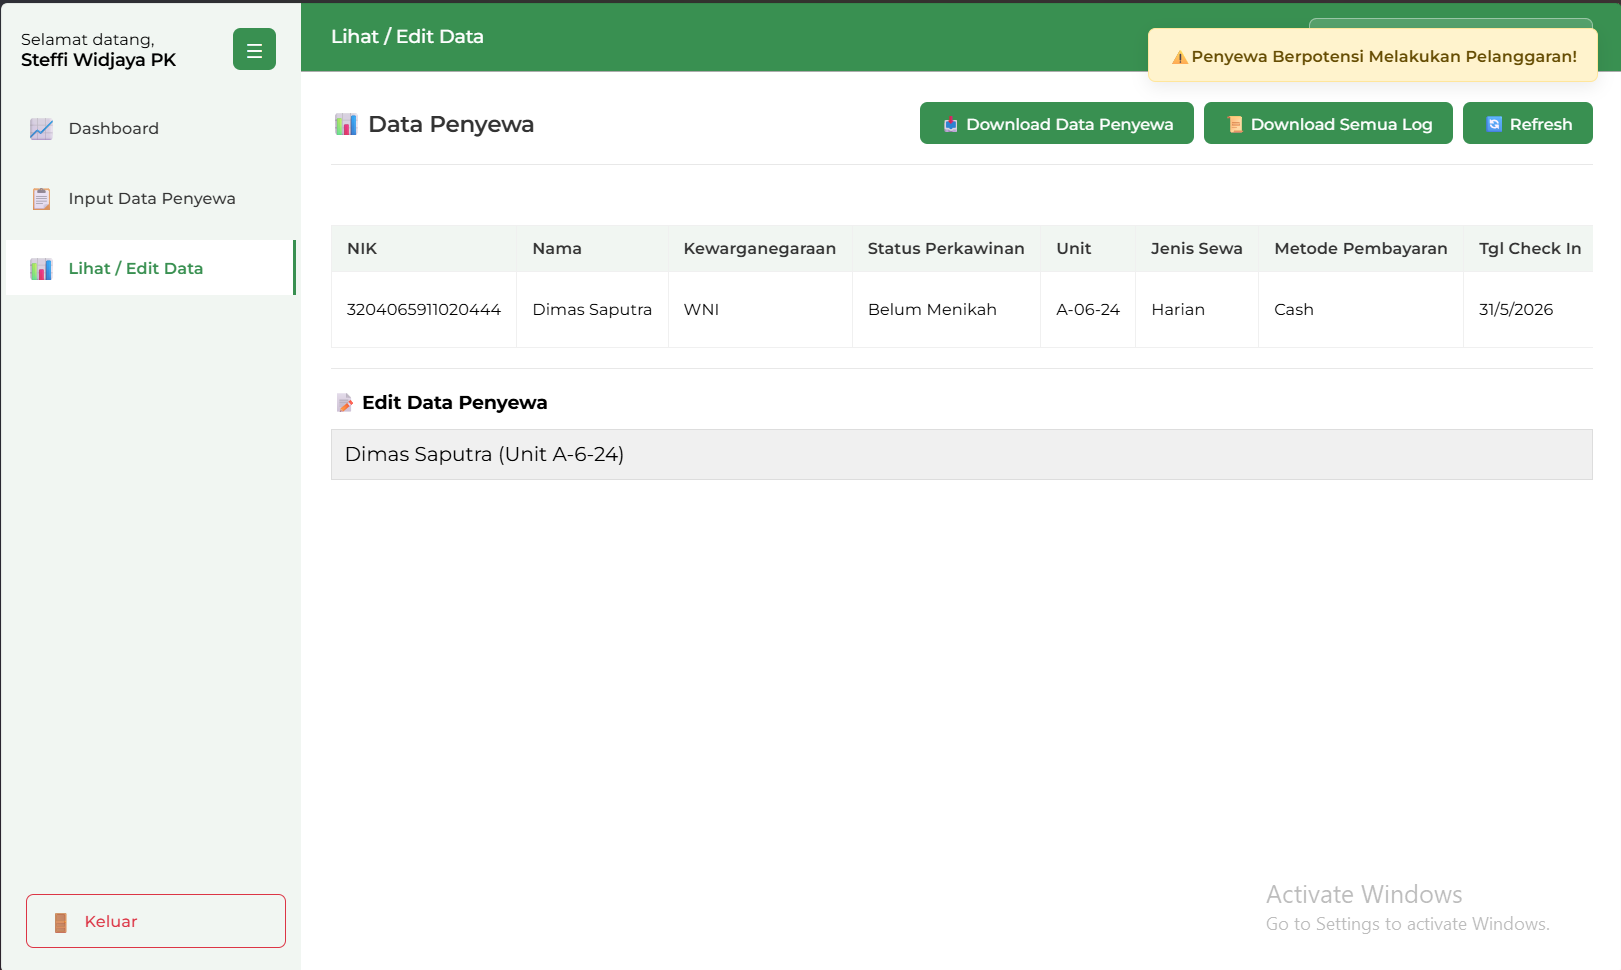
\includegraphics[width=0.7\textwidth]{Gambar/melanggar1b.png}
    \caption{Simulasi Input Data Penyewa Tidak Normal (1)}
    \label{fig:sim_input_tidak_normal1}
\end{figure}

\begin{figure}[H]
    \centering
    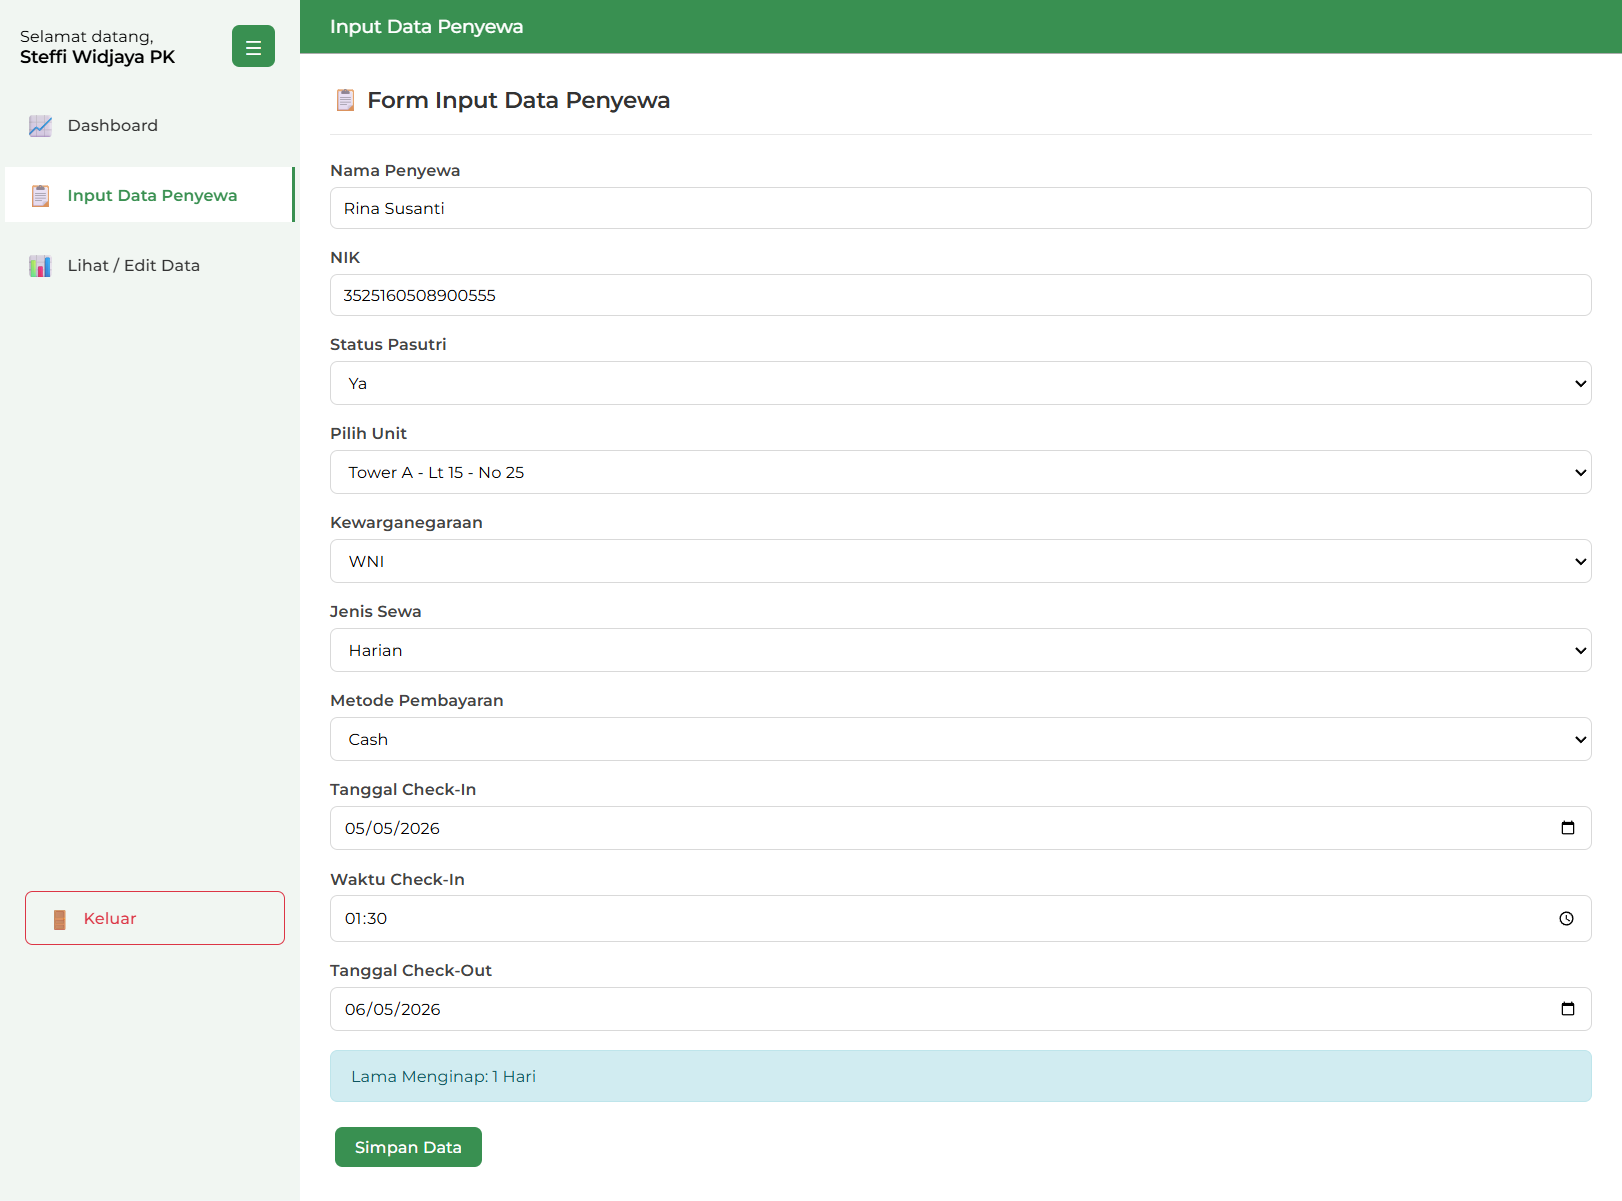
\includegraphics[width=0.7\textwidth]{Gambar/melanggar2a.png} \\
    \vspace{0.2cm}
    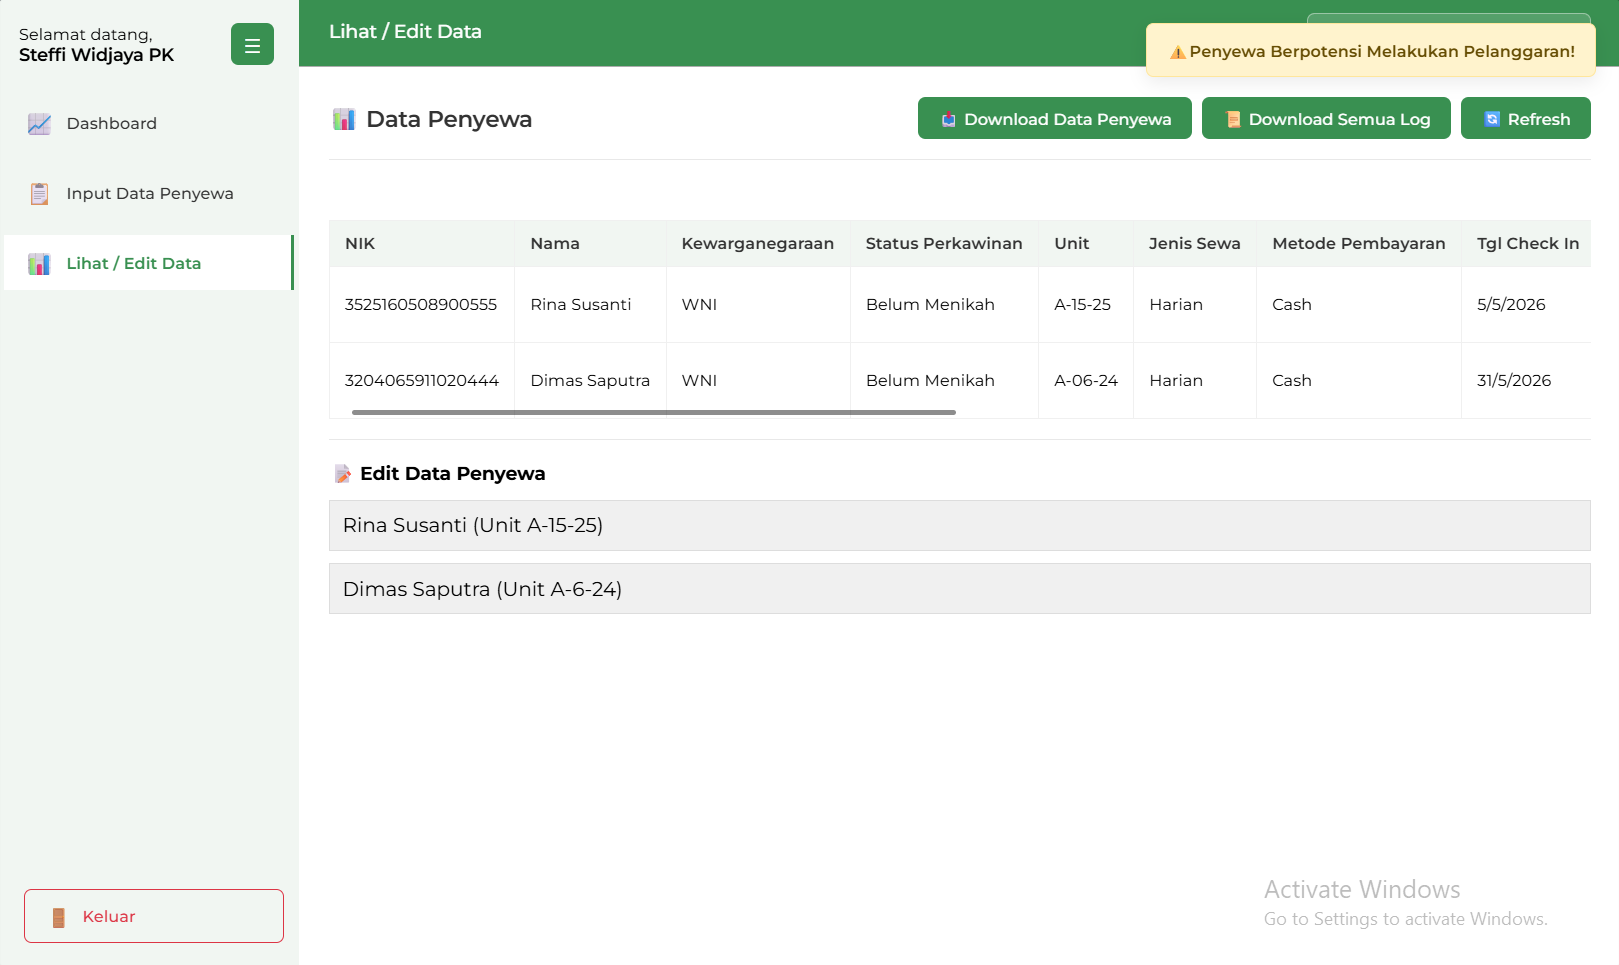
\includegraphics[width=0.7\textwidth]{Gambar/melanggar2b.png}
    \caption{Simulasi Input Data Penyewa Tidak Normal (2)}
    \label{fig:sim_input_tidak_normal2}
\end{figure}

\begin{figure}[H]
    \centering
    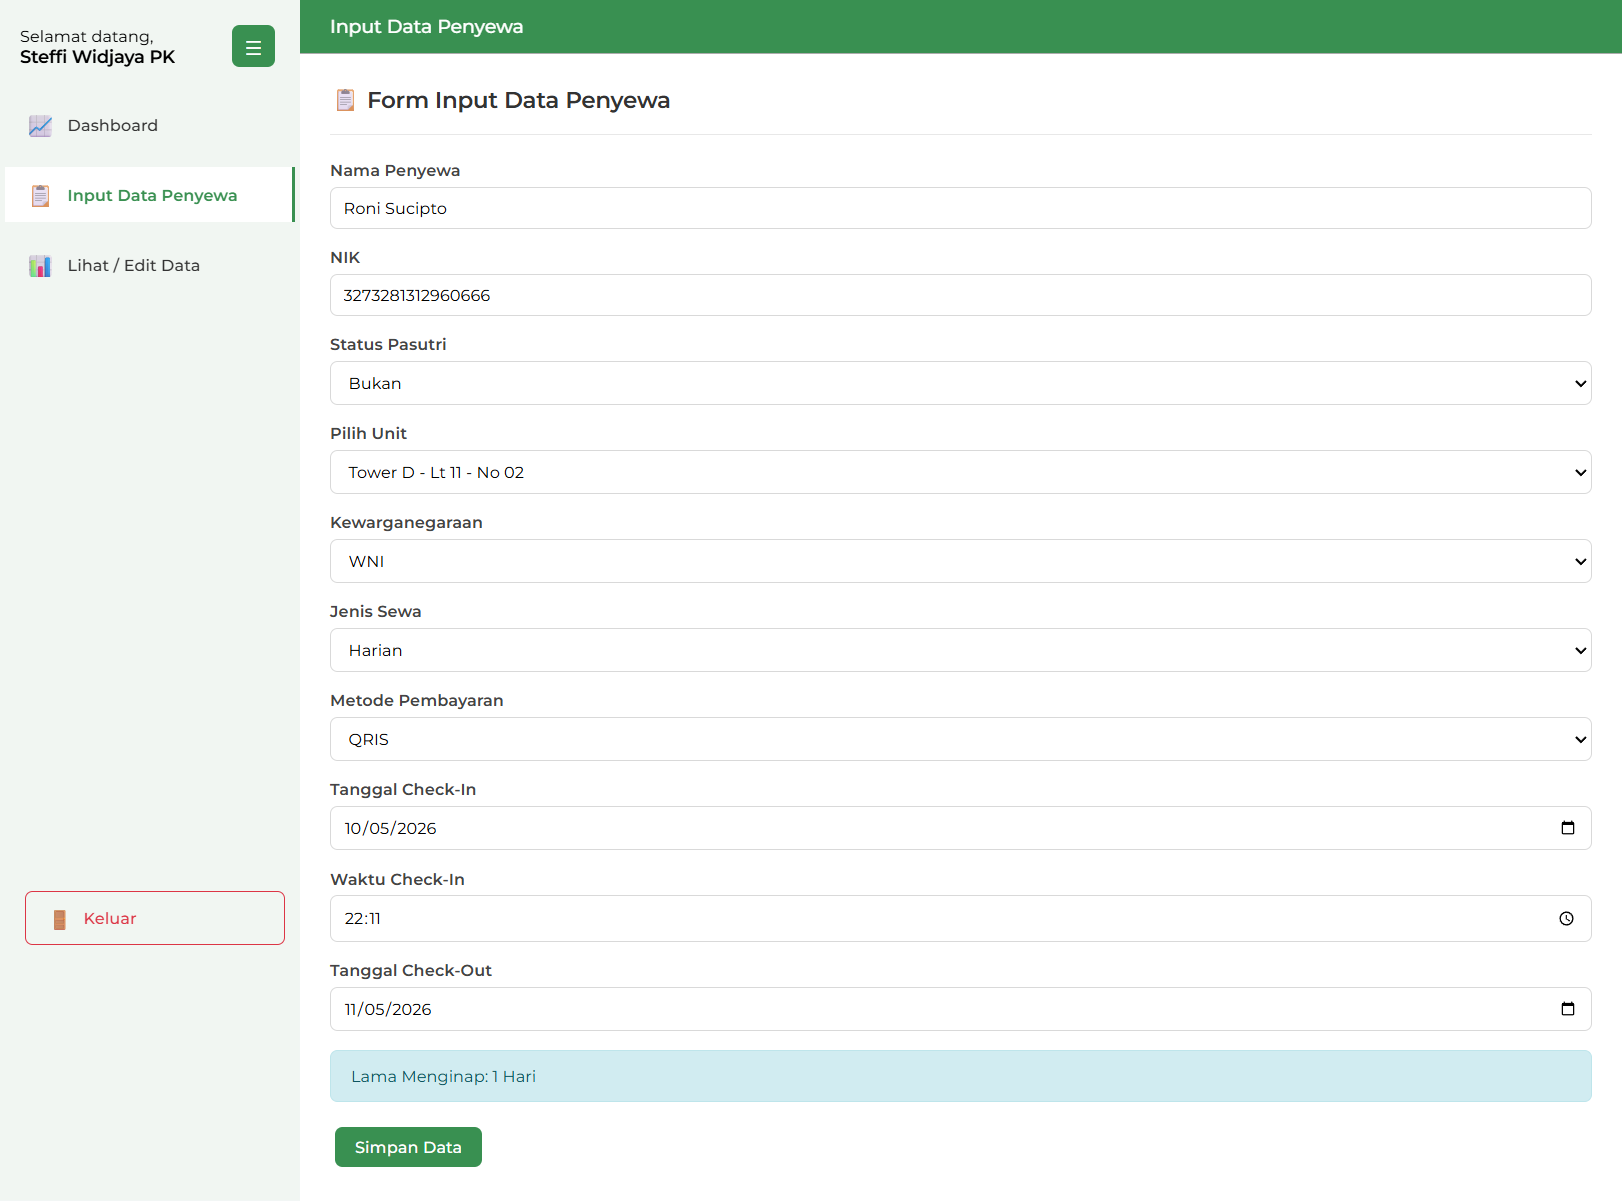
\includegraphics[width=0.7\textwidth]{Gambar/melanggar3a.png} \\
    \vspace{0.2cm}
    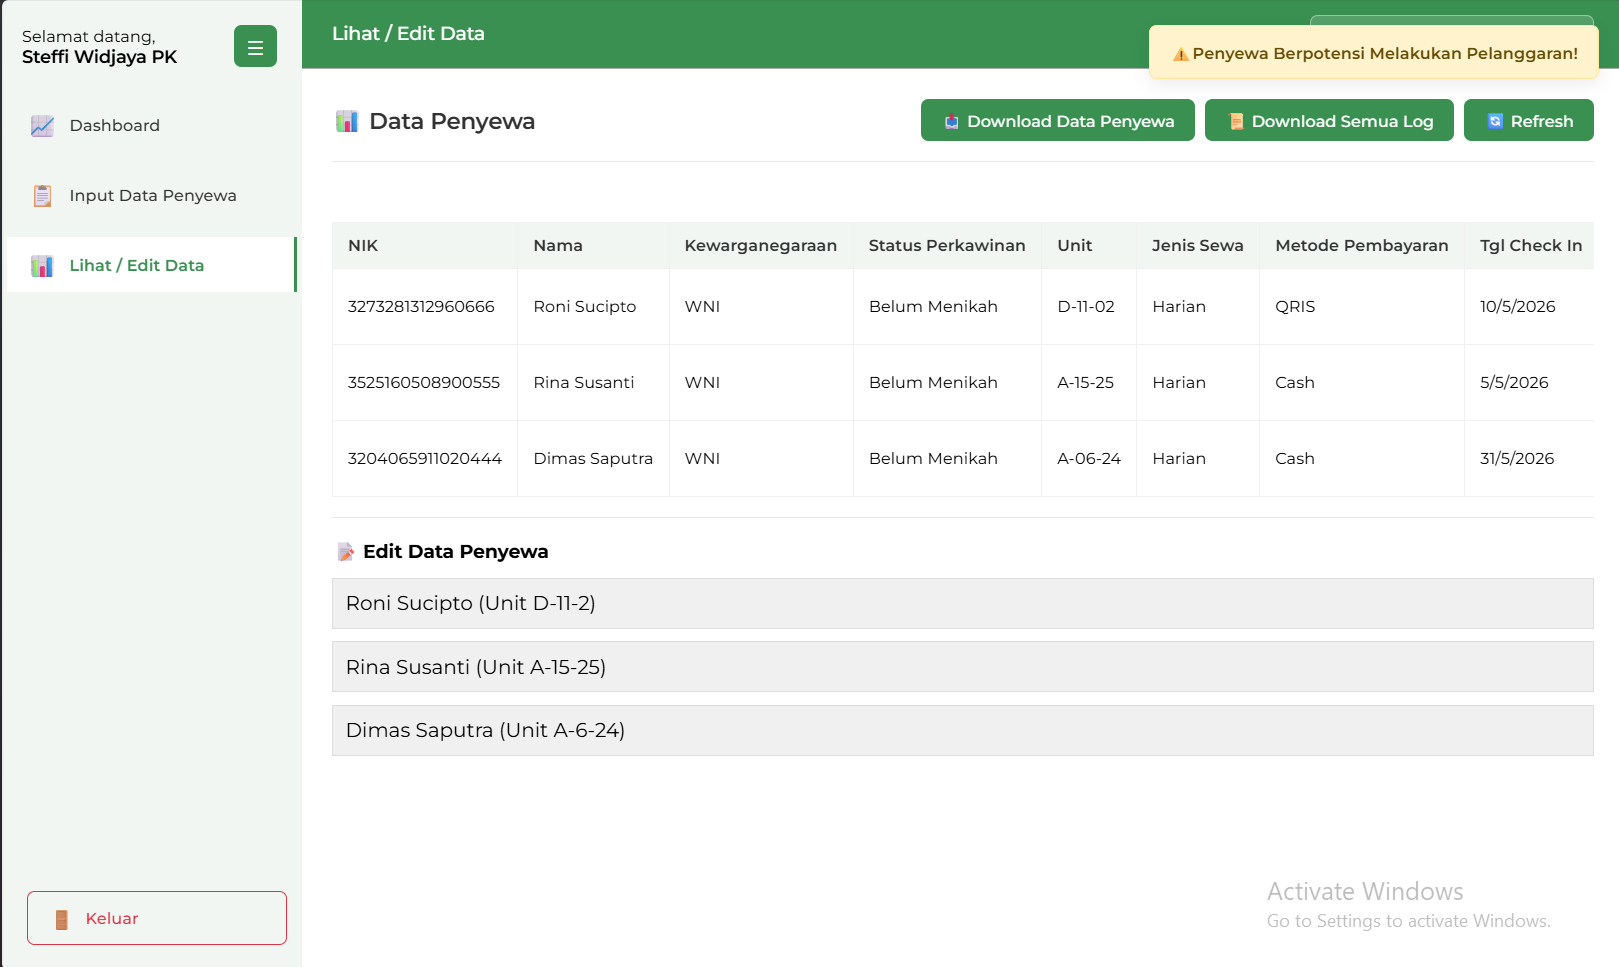
\includegraphics[width=0.7\textwidth]{Gambar/melanggar3b.png}
    \caption{Simulasi Input Data Penyewa Tidak Normal (3)}
    \label{fig:sim_input_tidak_normal3}
\end{figure}
\vspace{-0.5cm}
Gambar~\ref{fig:sim_input_tidak_normal1}, \ref{fig:sim_input_tidak_normal2}, dan \ref{fig:sim_input_tidak_normal3} memperlihatkan simulasi masukan data yang mengandung pola anomali. Penekanan pengisian difokuskan pada kombinasi atribut yang secara empiris menjadi karakteristik utama penyewa bermasalah pada tahapan analisis sebelumnya, seperti pemilihan jenis sewa harian yang dipadukan dengan durasi menginap yang sangat singkat (berkisar antara 0 hingga 1 hari). Setelah pengguna klik tombol \textit{Simpan Data}, aplikasi secara \textit{real-time} mentransmisikan sekumpulan data tersebut ke dalam model klasifikasi. Karena profil tersebut terdeteksi menyerupai karakteristik riwayat pelanggaran (terklasifikasi ke dalam kelas 1), maka aplikasi memberikan notifikasi berbunyi ``Penyewa Berpotensi Melakukan Pelanggaran!''. Peringatan ini bertujuan untuk langsung meningkatkan kewaspadaan Pengelola maupun Pelaku Komersil terhadap penyewa yang bersangkutan.


\subsection{Kesimpulan Hasil Pengujian}
Berdasarkan seluruh rangkaian pengujian fungsional aplikasi, pengujian integrasi, serta pengujian skenario peluncuran model di atas, dapat disimpulkan bahwa seluruh tahapan pengujian dan validasi sistem telah terlaksana dengan tuntas dan berjalan sesuai perancangan. Integrasi antara antarmuka aplikasi {data capture} dan model prediktif terbukti berfungsi secara optimal. Aplikasi mampu membaca, mengekstraksi, dan memproses setiap atribut data masukan pengguna secara \textit{real-time} untuk kemudian dianalisis oleh model klasifikasi secara akurat. Kepastian respons aplikasi yang presisi—berupa penyimpanan operasional yang mulus untuk profil aman serta intervensi notifikasi secara {\it real-time} untuk profil berisiko—menandakan bahwa seluruh fungsionalitas dan fitur pendeteksi dini (\textit{early warning system}) telah tervalidasi penuh serta siap dioperasikan sebagai instrumen pengawasan preventif pada kegiatan operasional penyewaan unit.